% Este trabalho está licenciado sob a licença Creative Commons CC-BY-SA.
% Você é livre para usar, compartilhar e adaptar este material, desde que seja atribuída a autoria e que as obras derivadas mantenham a mesma licença.

%--------------------ELEMENTOS PRÉ-TEXTUAIS--------------------%

%-----------------------------Capa-----------------------------%
\imprimircapa

%------------------------Folha de rosto------------------------%
\imprimirfolhaderosto


%----------------------Ficha Catalográfica----------------------%

\begin{fichacatalografica}
    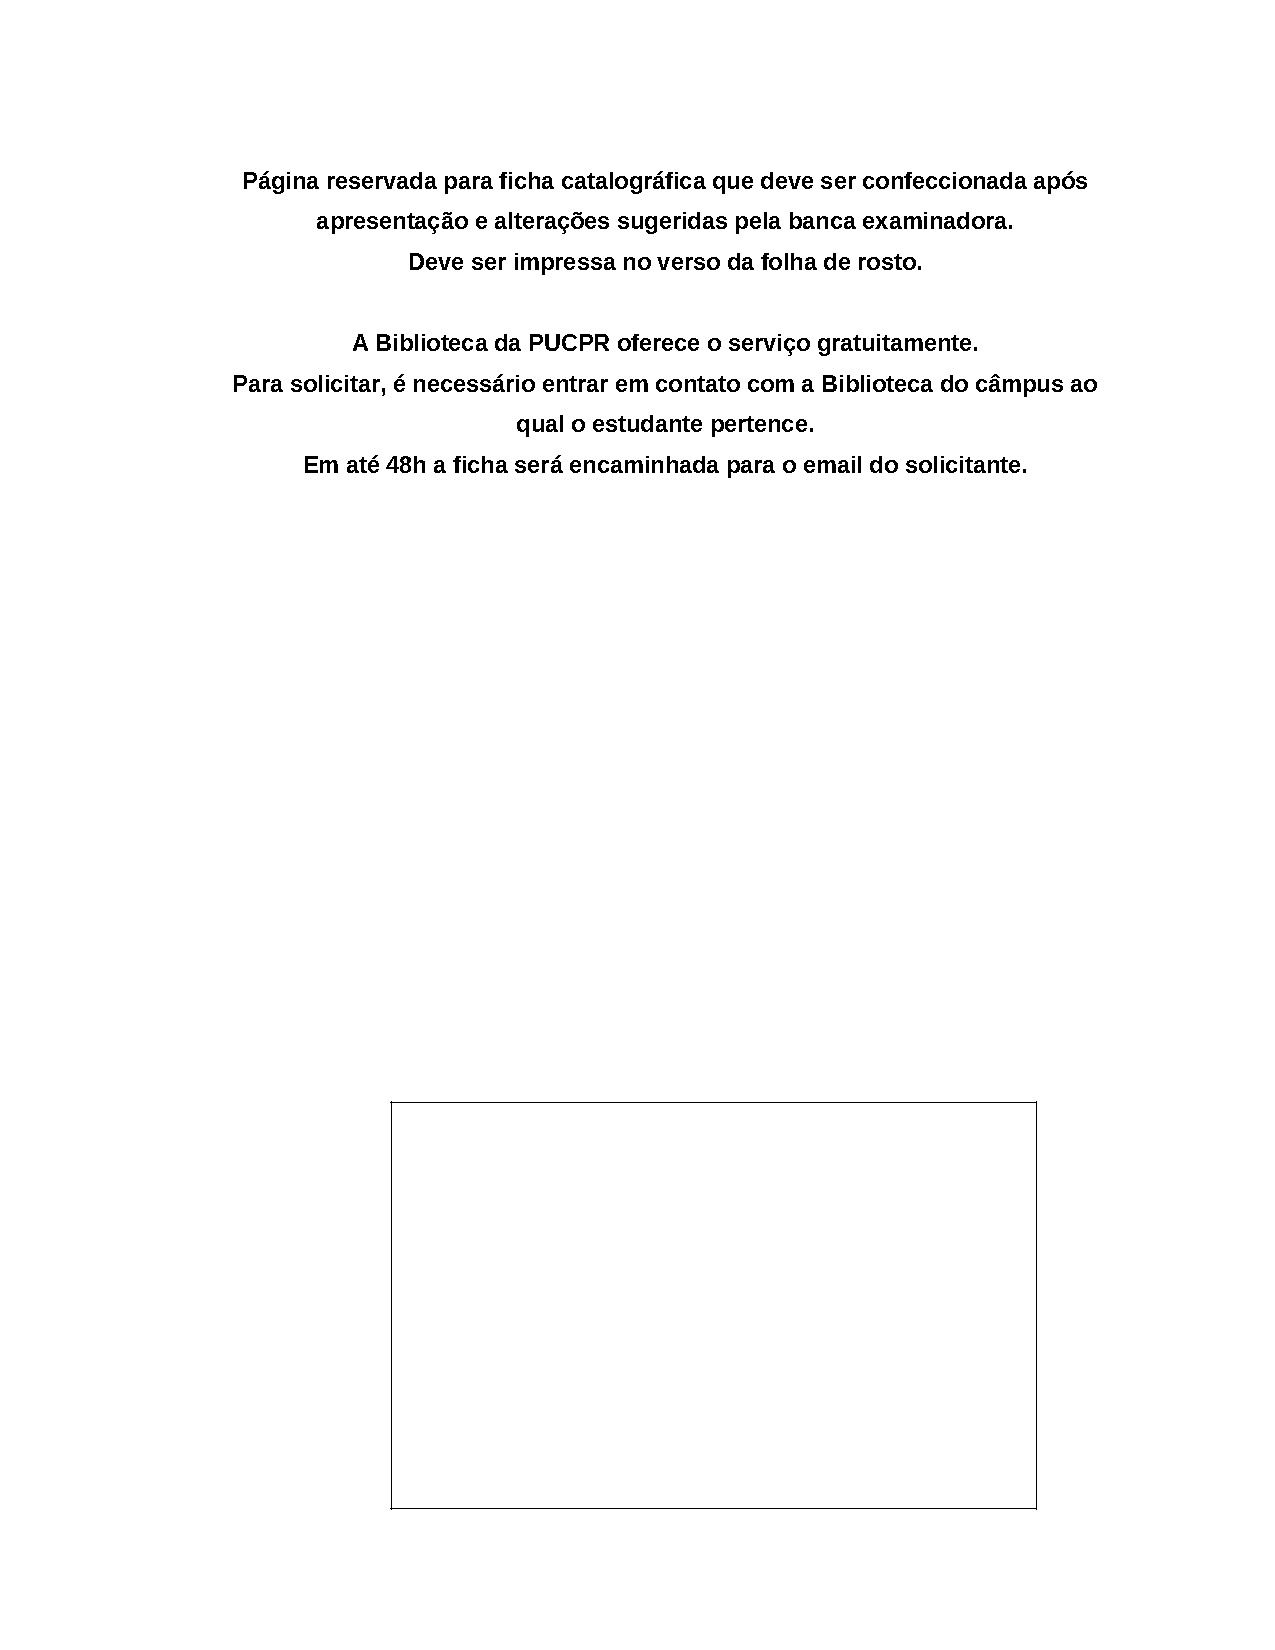
\includepdf{pdfs/ficha_catalografica.pdf}
\end{fichacatalografica}

%----------------------Folha de Aprovação----------------------%

% Após aprovação do trabalho, solicite do orientador a Folha de Aprovação assinada pela Banca Examinadora.
% Salve-a em formato PDF com o nome: folha_aprovacao.pdf
% Substitua o arquivo temporário de mesmo nome presente neste modelo.

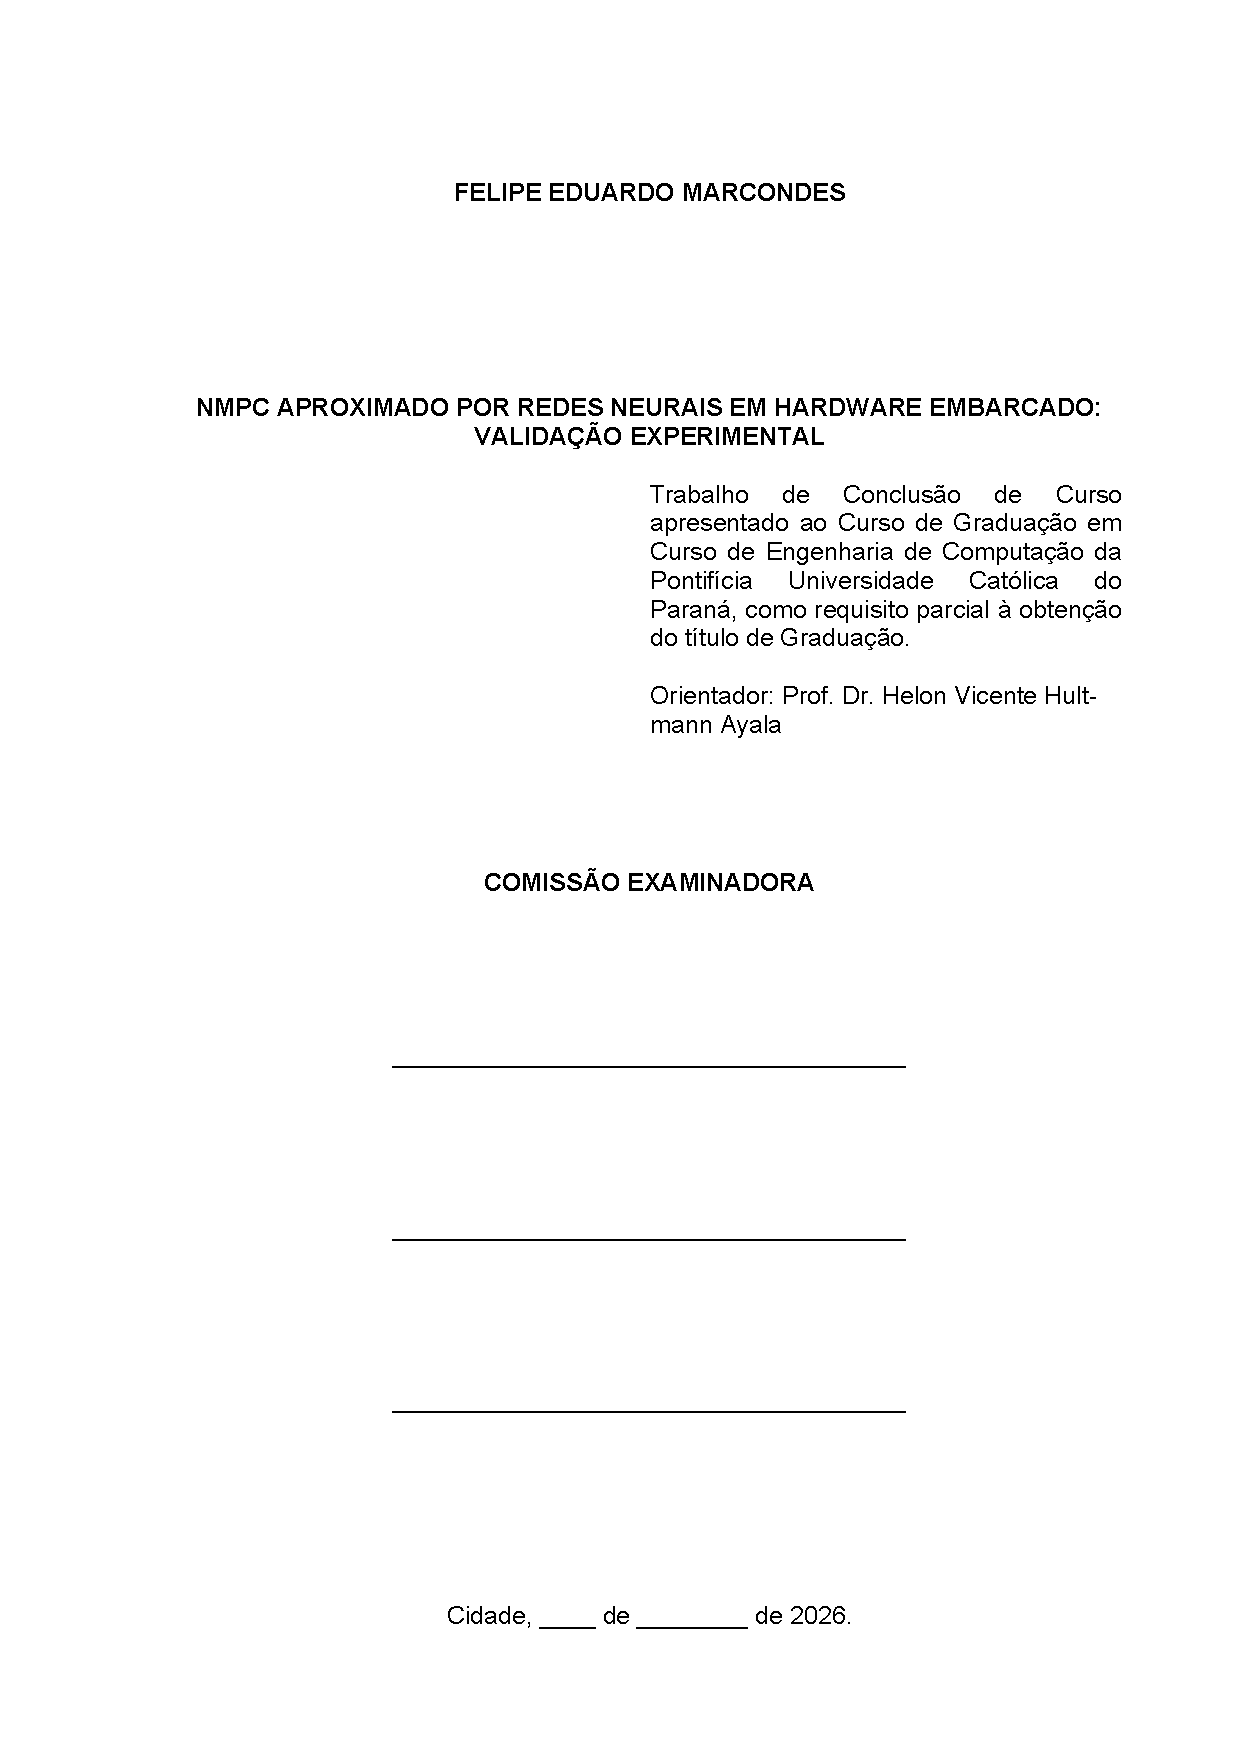
\includepdf{pdfs/folha-aprovacao.pdf}


%----------------------Dedicatória----------------------%
%\begin{dedicatoria}
%\vspace*{\fill}
%\begin{flushright}
%\begin{minipage}{8.5cm}
%\raggedleft
%\textit{
%A dedicatória deve ficar ao final da página e alinhada à direita.
%}
%\end{minipage}
%\end{flushright}
%\end{dedicatoria}



%----------------------Agradecimentos----------------------%
%\begin{agradecimentos}


%Agradeço à Pontifícia Universidade Católica do Paraná...

%Agradeço também ao órgão de fomento XYZ...  

%Sou grato(a) ao(à) meu(minha) orientador(a)... 

%Por fim, mas não menos importante, agradeço aos familiares e amigos...

%\end{agradecimentos}




%----------------------Epígrafe----------------------%
%\begin{epigrafe}
%    \vspace*{\fill}
%    \begin{flushright}
%        \begin{minipage}{8.5cm}
%            \raggedleft
%            \textit{}
%        \end{minipage}
%    \end{flushright}
%\end{epigrafe}


%----------------------Resumos----------------------%
%-%---------------Resumo em Português----------------%
\begin{resumo}
\SingleSpacing

    \noindent Este trabalho propõe o desenvolvimento e a validação experimental de um controlador neural embarcado para o rastreamento angular de um aeropêndulo instrumentado, visando contornar o elevado custo computacional do Controle Preditivo Não-Linear (NMPC) tradicional em microcontroladores. O sistema, operado por um motor BLDC e monitorado por uma IMU, é modelado fenomenologicamente e tem seus parâmetros aerodinâmicos e de atrito estimados experimentalmente pelo método de \textit{multiple shooting}. Um controlador PID estabiliza a planta na coleta de dados e serve como linha de base. A otimização iterativa do NMPC é substituída pela inferência direta de uma rede neural Perceptron Multicamadas (MLP), treinada em PyTorch com um conjunto de dados gerado pela resolução offline do problema de controle ótimo via CasADi. O modelo neural resultante é compilado em linguagem C nativa pela ferramenta X-CUBE-AI e executado em um microcontrolador STM32F446RE. O projeto avalia os compromissos entre a precisão do rastreamento de referências, a capacidade de rejeição a perturbações e as restrições de latência em tempo real ($T_s = 10$\,ms) e consumo de memória, comparando o desempenho da política neural embarcada com o controlador preditivo exato e a malha clássica.
    
    \vspace{\onelineskip}
    
    \noindent
    \textbf{Palavras-chave}: Aeropêndulo; Controle Preditivo Não-Linear; Redes Neurais Artificiais; Sistemas Embarcados; Identificação de Sistemas.
    
\end{resumo}

%----------------Resumo em Inglês----------------%
\begin{resumo}[\textbf{Abstract}]
\SingleSpacing
    \begin{otherlanguage*}{english}
    
        \noindent This work proposes the development and experimental validation of an embedded neural controller for the angular tracking of an instrumented aeropendulum, aiming to circumvent the high computational cost of traditional Nonlinear Model Predictive Control (NMPC) on microcontrollers. The system, driven by a BLDC motor and monitored by an IMU, is modeled phenomenologically and its aerodynamic and friction parameters are experimentally estimated using the multiple shooting method. A PID controller stabilizes the plant during data collection and serves as a baseline. The iterative optimization of the NMPC is replaced by the direct inference of a Multilayer Perceptron (MLP) neural network, trained in PyTorch with a dataset generated by the offline resolution of the optimal control problem via CasADi. The resulting neural model is compiled into native C code by the X-CUBE-AI tool and executed on an STM32F446RE microcontroller. The project evaluates the trade-offs between reference tracking accuracy, disturbance rejection capabilities, and the constraints of real-time latency ($T_s = 10$\,ms) and memory footprint, comparing the performance of the embedded neural policy with the exact predictive controller and the classical loop.
        
        \vspace{\onelineskip}
        
        \noindent 
        \textbf{Keywords}: Aeropendulum; Nonlinear Model Predictive Control; Artificial Neural Networks; Embedded Systems; System Identification.
        
    \end{otherlanguage*}
\end{resumo}




%----------------Lista de Ilustrações----------------%
\pdfbookmark[0]{\listfigurename}{lof}
\listoffigures*
\cleardoublepage


%----------------Lista de Quadros----------------%
\pdfbookmark[0]{\listofquadrosname}{loq}
\listofquadros*
\cleardoublepage




%----------------Lista de Tabelas----------------%
\pdfbookmark[0]{\listtablename}{lot}
\listoftables*
\cleardoublepage

%----------------Lista de Gráficos ----------------%
\pdfbookmark[0]{\listplotname}{lop}
\listofplots*
\cleardoublepage

%--------Lista de abreviaturas e siglas---------%
\begin{siglas}
    \item[ADC] Conversor Analógico-Digital (\textit{Analog-to-Digital Converter})
    \item[BLDC] Motor de Corrente Contínua sem Escovas (\textit{Brushless Direct Current})
    \item[CLF] Função de Lyapunov de Controle (\textit{Control Lyapunov Function})
    \item[DAG] Grafo Direcionado Acíclico (\textit{Directed Acyclic Graph} / Grafo de expressão simbólica)
    \item[Diffrax] Biblioteca para solução numérica diferenciável de equações diferenciais
    \item[DLPF] Filtro Passa-Baixas Digital (\textit{Digital Low-Pass Filter})
    \item[DMA] Acesso Direto à Memória (\textit{Direct Memory Access})
    \item[DNN] Rede Neural Profunda (\textit{Deep Neural Network})
    \item[dps] Graus por segundo (\textit{degrees per second})
    \item[EMPC] Controle Preditivo Baseado em Modelo Explícito (\textit{Explicit MPC})
    \item[ESC] Controlador Eletrônico de Velocidade (\textit{Electronic Speed Controller})
    \item[FFNN] Rede Neural \textit{Feedforward} (\textit{Feedforward Neural Network})
    \item[FPU] Unidade de Ponto Flutuante (\textit{Floating-Point Unit})
    \item[I$^2$C] \textit{Inter-Integrated Circuit}
    \item[IMU] Unidade de Medição Inercial (\textit{Inertial Measurement Unit})
    \item[JAX] Estrutura computacional para diferenciação automática e computação numérica de alta performance
    \item[MAE] Erro Absoluto Médio (\textit{Mean Absolute Error})
    \item[MCU] Microcontrolador (\textit{Microcontroller Unit})
    \item[MDF] \textit{Medium Density Fiberboard}
    \item[MEMS] Sistemas Microeletromecânicos (\textit{Micro-Electro-Mechanical Systems})
    \item[MLP] Perceptron Multicamadas (\textit{Multilayer Perceptron})
    \item[MPC] Controle Preditivo Baseado em Modelo (\textit{Model Predictive Control})
    \item[MSE] Erro Quadrático Médio (\textit{Mean Squared Error})
    \item[NLP] Programação Não-Linear (\textit{Nonlinear Programming})
    \item[NMPC] Controle Preditivo Não-Linear (\textit{Nonlinear Model Predictive Control})
    \item[OCP] Problema de Controle Ótimo (\textit{Optimal Control Problem})
    \item[ODE] Equação Diferencial Ordinária (\textit{Ordinary Differential Equation})
    \item[PID] Proporcional-Integral-Derivativo
    \item[PINN] Rede Neural Informada pela Física (\textit{Physics-Informed Neural Network})
    \item[PLA] Poliácido Láctico
    \item[PWA] Função Afim por Partes (\textit{Piecewise Affine})
    \item[PWM] Modulação por Largura de Pulso (\textit{Pulse Width Modulation})
    \item[QFN] \textit{Quad Flat No-leads}
    \item[ReLU] Unidade Linear Retificada (\textit{Rectified Linear Unit})
    \item[RMSE] Raiz do Erro Quadrático Médio (\textit{Root Mean Square Error})
    \item[SLSQP] Programação Sequencial de Mínimos Quadrados (\textit{Sequential Least Squares Programming})
    \item[SRAM] Memória de Acesso Aleatório Estática (\textit{Static Random Access Memory})
    \item[TCC] Trabalho de Conclusão de Curso
    \item[TFLM] TensorFlow Lite Micro
    \item[TIM] Temporizador (\textit{Timer})
    \item[UART] Transmissor-Receptor Assíncrono Universal (\textit{Universal Asynchronous Receiver-Transmitter})
    \item[USART] Transmissor-Receptor Síncrono e Assíncrono Universal (\textit{Universal Synchronous and Asynchronous Receiver-Transmitter})
    \item[VANT] Veículo Aéreo Não Tripulado
    \item[VTOL] Decolagem e Aterrissagem Vertical (\textit{Vertical Take-Off and Landing})
    \item[ZOH] Segurador de Ordem Zero (\textit{Zero-Order Hold})
\end{siglas}

%----------------Lista de Símbolos----------------%
\begin{simbolos}
    \item[$ \alpha $] Fator do filtro complementar
    \item[$ b $] Coeficiente de atrito viscoso
    \item[$ \mathcal{D} $] Conjunto de dados (\textit{dataset}) de treinamento
    \item[$ e $] Erro de rastreamento
    \item[$ f(\cdot) $] Função de transição de estados (dinâmica não-linear)
    \item[$ g $] Aceleração da gravidade
    \item[$ J $] Momento de inércia total do aeropêndulo
    \item[$ K_p, K_i, K_d $] Ganhos proporcional, integral e derivativo do controlador PID
    \item[$ K_\tau $] Constante de empuxo do motor
    \item[$ \kappa_N(\cdot) $] Lei de controle implícita do NMPC
    \item[$ L_1 $] Distância do conjunto motor-hélice ao pivô de rotação
    \item[$ L_2 $] Distância do contrapeso ao pivô de rotação
    \item[$ \ell(\cdot) $] Função de custo de estágio
    \item[$ M $] Número de intervalos no método \textit{multiple shooting}
    \item[$ m_1 $] Massa do conjunto motor-hélice
    \item[$ m_2 $] Massa do contrapeso
    \item[$ N $] Horizonte de predição
    \item[$ P $] Matriz de peso do custo terminal
    \item[$ Q $] Matriz de peso dos estados no custo de estágio
    \item[$ R $] Matriz de peso da ação de controle no custo de estágio
    \item[$ r $] Sinal de referência
    \item[$ s_i $] Variável de estado inicial local no método \textit{multiple shooting}
    \item[$ \theta $] Posição angular do braço do aeropêndulo
    \item[$ \dot{\theta} $] Velocidade angular
    \item[$ \ddot{\theta} $] Aceleração angular
    \item[$ \hat{\theta} $] Vetor de parâmetros a estimar
    \item[$ T_s $] Período de amostragem
    \item[$ \tau $] Torque gerado pelo empuxo do motor
    \item[$ U_k $] Sequência de controle a otimizar
    \item[$ u $] Sinal de controle (\textit{duty cycle} do PWM)
    \item[$ V_f(\cdot) $] Função de custo terminal
    \item[$ V_N^0(\cdot) $] Função de valor ótimo
    \item[$ x $] Vetor de estados do sistema
    \item[$ \mathcal{X} $] Conjunto admissível de estados / Conjunto de variáveis de decisão
    \item[$ \mathcal{X}_f $] Conjunto terminal
    \item[$ \mathcal{X}_N $] Domínio de factibilidade do Problema de Controle Ótimo
    \item[$ y $] Variável de processo observada
\end{simbolos}


%----------------SUMÁRIO----------------%
\pdfbookmark[0]{\contentsname}{toc}
\tableofcontents*
\cleardoublepage